\documentclass[12pt]{article}
\usepackage{a4wide}
\usepackage{latexsym}
\usepackage{amssymb}
\usepackage{epic}
\usepackage{amsmath}
\usepackage{graphicx}
\usepackage{comment}
\usepackage{graphicx}
\usepackage{tikz}
%\pagestyle{empty}
\newcommand{\tr}{\mbox{\sf true}}
\newcommand{\fa}{\mbox{\sf false}}
\newcommand{\bimp}{\leftrightarrow}

\begin{document}
\section*{Automated Reasoning\\Extra Assignment}

\begin{center}
Judith van Stegeren (s3014827)\\
\end{center}

\vspace{8mm}

\subsection*{Red-blue-paths}
\paragraph{The problem}
In an undirected network the edges are colored red and blue:\\
\begin{center}
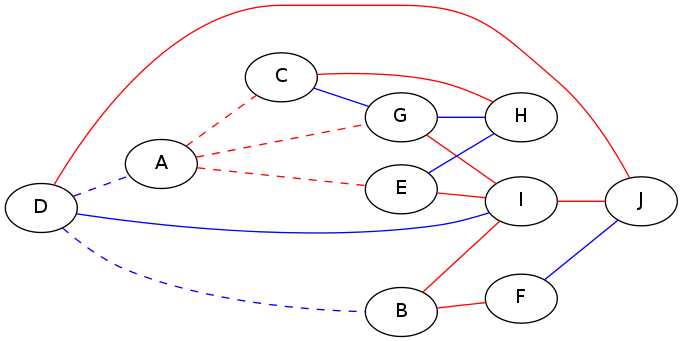
\includegraphics[width=12cm]{graph.png}\\
\end{center}
For each color, only one of the dashed edges exists: we do not know which one.
Prove that there is a path from A to B in which no two consecutive edges are of the same color.

\paragraph{Solution}
We start out by defining predicates:
\begin{enumerate} 
\item \texttt{red(a,b)} means that there is an edge between nodes $a$ and $b$ with the color red. 
\item \texttt{blue(a,b)} means that there is an edge between nodes $a$ and $b$ with the color blue.
\item \texttt{rp(a,b)} means that there is a path between $a$ and $b$, of which no two consecutive edges are the same color and where the final edge is colored red.
\item \texttt{bp(a,b)} means that there is a path between $a$ and $b$, of which no two consecutive edges are the same color and where the final edge is colored blue.
\end{enumerate}

We want the edges to be two-ways, since this is an undirected graph:
\begin{verbatim}
blue(x,y) -> blue(y,x).
red(x,y) -> red(y,x).
\end{verbatim}

We construct the notion of a valid path (in which no two consecutive edges are the same color) as follows:

If there is a red/blue edge between $x$ and $y$ then there is also a valid path between $x$ and $y$, in which no two consecutive edges are the same color, that ends in a red/blue edge:
\begin{verbatim}
blue(x,y) -> bp(x,y).
red(x,y) -> rp(x,y).
\end{verbatim}

If there is a valid path between nodes $x$ and $y$ that ends with a red edge, and there is an edge between $y$ and $z$ that is coloured blue, we can make a new valid path between $x$ and $z$ that ends with blue:
\[ \texttt{(rp(x,y) \& blue(y,z)) -> bp(x,z).}\]
The same thing holds for a valid path between nodes $x$ and $y$ that ends with blue: if there is an edge between $y$ and $z$ that is coloured red, we can make a new valid path between $x$ and $z$ that ends with a red edge:
\[ \texttt{(bp(x,y) \& red(y,z)) -> rp(x,z).} \]

We can now specify the graph with these new predicates. First, we add all given edges of the graph as assumptions:
\begin{verbatim}
% red edges:
red(b,f) & red(b,i) & red(c,h) & red(d,j) & red(e,i) & red(g,i) & red(i,j).
% blue edges:
blue(c,g) & blue(d,i) & blue(e,h) & blue(f,j) & blue(g,h).
\end{verbatim}

\subsection*{Part A}
Now we add the special edges as assumptions.
There is only one of the edges AC, AE, AG and only one of the edges DA and DB:
\begin{verbatim}
% RED EDGES
% one of AC, AE, AG
red(a,c) | red(a,e) | red(a,g).
% not all three at the same time
-( red(a,c) & red(a,e) & red(a,g) ).
% not two at the same time
-( red(a,c) & red(a,e) ).
-( red(a,c) & red(a,g) ).
-( red(a,e) & red(a,g) ).

% BLUE EDGES
% one of DA, DB
blue(d,a) | blue(d,b).
% not both
-( blue(d,a) & blue(d,b) ).
\end{verbatim}

To find our whether there is a valid path between $a$ and $b$, we ask prover9 to prove the following goal:
\[ \texttt{rp(a,b) | bp(a,b)} \]

Prover9 returned \texttt{THEOREM PROVED} within a second.

\subsection*{Part B}
We know now that edges AE and DB exist.
We remove the code that deals with the special edges and add the two given edges instead:
\begin{verbatim}
red(a,e).
blue(d,b).
\end{verbatim}
If we ask prover9 to solve either \texttt{bp(a,b) | rp(a,b)} or \texttt{bp(a,b)}, prover9 takes a long time. If we ask prover9 to solve \texttt{rp(a,b)} instead, we get a \texttt{THEOREM PROVED} within a second. 
According to the output of prover 9, this is the path between A and B:\\

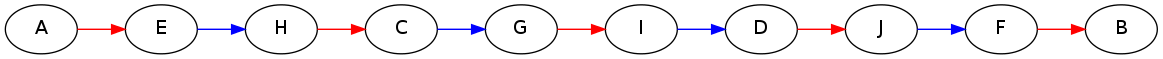
\includegraphics[width=16cm]{path.png}\\

We found this path by looking at the prover9 output under \texttt{PROOF}, where we found the following list of edges:
\begin{verbatim}
16 red(a,e).  [assumption].
17 red(b,f).  [clausify(7)].
19 red(c,h).  [clausify(7)].
20 red(d,j).  [clausify(7)].
22 red(g,i).  [clausify(7)].
25 blue(c,g).  [clausify(8)].
26 blue(d,i).  [clausify(8)].
27 blue(e,h).  [clausify(8)].
28 blue(f,j).  [clausify(8)].
\end{verbatim}
It was not hard to reconstruct the path from this list.

\clearpage{}

\section*{Appendix A: prover9 code exercise A}
\begin{verbatim}
formulas(assumptions).
blue(x,y) -> blue(y,x).
red(x,y) -> red(y,x).
	
blue(x,y) -> bp(x,y).
red(x,y) -> rp(x,y).

(bp(x,y) & red(y,z)) -> rp(x,z).
(rp(x,y) & blue(y,z)) -> bp(x,z).

red(a,c) | red(a,e) | red(a,g).
-( red(a,c) & red(a,e) & red(a,g) ).
-( red(a,c) & red(a,e) ).
-( red(a,c) & red(a,g) ).
-( red(a,e) & red(a,g) ).

red(b,f) & red(b,i) & red(c,h) & red(d,j) & red(e,i) & red(g,i) & red(i,j).

blue(d,a) | blue(d,b).
-( blue(d,a) & blue(d,b) ).

blue(c,g) & blue(d,i) & blue(e,h) & blue(f,j) & blue(g,h).
	
end_of_list.

formulas(goals).
	rp(a,b) | bp(a,b).
end_of_list.
\end{verbatim}

\clearpage{}

\section*{Appendix B: prover9 code exercise B}
\begin{verbatim}
formulas(assumptions).
blue(x,y) -> blue(y,x).
red(x,y) -> red(y,x).
	
blue(x,y) -> bp(x,y).
red(x,y) -> rp(x,y).

(bp(x,y) & red(y,z)) -> rp(x,z).
(rp(x,y) & blue(y,z)) -> bp(x,z).

red(a,e).

red(b,f) & red(b,i) & red(c,h) & red(d,j) & red(e,i) & red(g,i) & red(i,j).

blue(d,b).

blue(c,g) & blue(d,i) & blue(e,h) & blue(f,j) & blue(g,h).
	
end_of_list.

formulas(goals).
	rp(a,b).
end_of_list.
\end{verbatim}




%\bibliography{report}{}
%\bibliographystyle{plain}

\end{document}
